\documentclass[12pt, a4paper, notitlepage]{report}
\usepackage{mathptmx}
\usepackage[T1]{fontenc}
\usepackage[utf8x]{inputenc}
\usepackage[english]{babel}
\usepackage{graphicx}
\usepackage{float}
\usepackage{amsmath}
\usepackage{mathtools}
\usepackage{amsfonts}
\usepackage{enumerate}
\usepackage{subfigure}
\usepackage[caption = false]{subfig}
\usepackage[top=2.5cm, bottom=2.5cm, left=2cm, right=2cm]{geometry}
\usepackage[font={small,it}]{caption}
\usepackage{fancyhdr}
\usepackage{listings}
\usepackage{color}
\usepackage{verbatim}

%\graphicspath{ {./Res\_L5\_k10/} {./Res\_L5\_k100/} {./Res\_L5\_k1000/} {./Res\_L10\_k10/} {./Res\_L10\_k100/} {./Res\_L10\_k1000/} {./Res\_L15\_k10/} {./Res\_L15\_k100/} {./Res\_L15\_k1000/} }

\definecolor{dkgreen}{rgb}{0,0.6,0}
\definecolor{gray}{rgb}{0.5,0.5,0.5}
\definecolor{mauve}{rgb}{0.58,0,0.82}
\definecolor{lyellow}{rgb}{1,1,0.9}

\lstset{backgroundcolor=\color{lyellow},
	frame=tb,
	language=Fortran,
	aboveskip=3mm,
	belowskip=3mm,
	showstringspaces=false,
	columns=flexible,
	basicstyle={\small\ttfamily},
	numbers=none,
	numberstyle=\tiny\color{gray},
	keywordstyle=\color{blue},
	commentstyle=\color{dkgreen},
	stringstyle=\color{mauve},
	breaklines=true,
	breakatwhitespace=true,
	tabsize=3
}

\pagestyle{fancy}
\lhead{Tommaso Tabarelli}
\chead{\thepage}
\rhead{\today}
\cfoot{Information theory and computation}
\rfoot{A.y. 2019/2020}
\lfoot{Exercise 10}

\begin{document}

\begin{center}
	\LARGE{Quantum information and computation: homework 10}\\
	\Large{of Tommaso Tabarelli}
\end{center}


\begin{abstract}
	In this homework we are asked to evaluate the ground state of a system of N spin-1/2 particles in a one-dimensional lattice using the \textit{real-space Renormalization Group} algorithm. We should write the given Hamiltonian in a proper form and draw conclusions analyzing its spectrum (for $N \to \infty$, thus iterating the procedure).
\end{abstract}

\section*{Theory}

The N spin-1/2 particles system is described by the following hamiltonian:
\begin{equation}
\hat{H} = \lambda \sum_{i}^{N} \hat{\sigma}_z^i + \sum_{i}^{N-1} \hat{\sigma}_x^i \hat{\sigma}_x^{i+1}
\end{equation}
To be able to write down the hamiltonian in a matrix form, a basis shuold be chosen. For simplicity of representation, the z-component spin basis was chosen. Thus, it holds:
\begin{equation}
	\hat{\sigma}_z = \left(
	\begin{matrix}
		1 & 0 \\
		0 & -1
	\end{matrix} \right)
	\quad
	\hat{\sigma}_x = \left(
	\begin{matrix}
		0 & 1 \\
		1 & 0
	\end{matrix}
	\right)
\end{equation}
To go on, an important fact to notice is the implicit dimension of the $\sigma$s: every spin is implicitely immerged in the whole system space, thus it is represented by the tensor product between the identity matrices of other subsystems (the other particles) $\mathbb{I}_2^i$ and its own spin operator $\sigma_{x/z}$:
\begin{equation}
\sigma_z^i = \mathbb{I}^1 \otimes \mathbb{I}^2 \otimes ... \otimes \sigma_z^i \otimes ... \otimes \mathbb{I}^N
\end{equation}
Using the same argument, the interaction term results:
\begin{equation}
	\sigma_x^i \sigma_x^{i+1} = \mathbb{I}^1 \otimes \mathbb{I}^2 \otimes ... \otimes \sigma_x^i \otimes \sigma_x^{i+1} \otimes ... \otimes \mathbb{I}^N
\end{equation}

The system is not separable. To evaluate the ground state we will use the \textit{real-space renormalization group} algorithm:
\begin{itemize}
	\item The starting point is a system of size N; in this case, the Hamiltonian should be $H_N:\mathbb{C}^d \to \mathbb{C}^d$, where $d$ is the dimension of the system composed by $N$ subsystems, thus $d=dim^N$, where $dim$ is the dimension of a single subsystem (a single particle) and it is supposed to be the same for every subsystem.
	
	\item Next step is to build a compound system of size 2N, "duplicating" the system described by $H_N$ and making the two subsystems (conventionally named A and B) interact (in this case, using \textit{nearest neighbours} interaction involving the particles which are located at the boundaries of the subsystems, thus the "rightmost" particle in the system A, which is "on the left", and the "leftmost" particle of system B).
	\begin{equation}
		H_{2N} = H^A_N + H^B_N + H^{AB}
	\end{equation}
	Notice that this writing has some implicit dimension handling, indeed $H_{2N}:\mathbb{C}^{d^2} \to \mathbb{C}^{d^2}$ and the other pieces have to be intended as follows:
	\begin{itemize}
		\item $H^A_N:\mathbb{C}^d \to \mathbb{C}^d \quad \Rightarrow \quad H^A_N \otimes \mathbb{I}^B_N : \mathbb{C}^{d^2} \to \mathbb{C}^{d^2}$
		\item $H^B_N:\mathbb{C}^d \to \mathbb{C}^d \quad \Rightarrow \quad \mathbb{I}^A_N \otimes H^B_N : \mathbb{C}^{d^2} \to \mathbb{C}^{d^2}$
		\item $H^{AB} = (\mathbb{I}^{\otimes N-1} \otimes \sigma_x)^A \otimes (\sigma_x \otimes \mathbb{I}^{\otimes N-1})^B $
	\end{itemize}

	\item The main idea is now to diagonalize the matrix $H_{2N}$ keeping only the first $d$ dimension (thus, $dim^{N}$, where $dim$ is the dimension of a "single particle system"). To do it, the eigenvector matrix is needed: $V \in \mathbb{M}(d^2,d^2)$. To make the proper truncation, we need to take only the first $d$ eigenvectors $P \equiv V^{trunc} \in \mathbb{M}(d^2,d)$ (which corresponds to the first $d$ eigenvalues taken in ascending order) and use them to project the hamiltonian $H_{2N}$ into a lower dimensional space.
	\begin{equation}
		H^{trunc}_{2N} = P^{\dagger} \cdot H_{2N} \cdot P
	\end{equation}
	
	\item Next step is to iterate the previous points, taking into account that the transformation of $H^{AB}$ is as following:
	\begin{equation}
		H^{AB}_{next\ step} = P^{\dagger} \left[ \mathbb{I}^{N-1} \otimes \sigma_N \otimes \mathbb{I}^N \right] \cdot P \otimes P^{\dagger} \cdot \left[ \mathbb{I}^{N} \otimes \sigma_1 \otimes \mathbb{I}^{N-1} \right] \cdot P
	\end{equation}
	so both matrices need first to be transformed and then to be used as before (remember that $P$ matrix acts a truncation, so the tensor product between the two transformed matrices restores the dimension to $d^2$).
\end{itemize}

Using a \textit{mean field} approximation we can estimate the ground state energy of the system. In this framework it holds:
\begin{equation}
	E[\psi_{MF}] = \langle \psi_{MF} \rvert H \lvert \psi_{MF} \rvert = \sum_{j=1}^{N-1} \langle \psi_{MF} \rvert \sigma_x^j \lvert \psi_{MF} \rangle^2 + \lambda \sum_{i=1}^{N} \langle \psi_{MF} \rvert \sigma_z^i \lvert \psi_{MF} \rangle
\end{equation}
and, in the termodynamic limit $N \to \infty$ it holds:
\begin{equation}
	e[\psi] = \frac{E[\psi]}{N} \underset{N \to \infty}{=} \langle \psi_{MF} \rvert \sigma_x \lvert \psi_{MF} \rangle^2 + \lambda \langle \psi_{MF} \rvert \sigma_z \lvert \psi_{MF} \rangle
\end{equation}
To find the ground state of the system the minimum of this quantity has to be find. It is found that:
\begin{equation}
	e = \begin{cases}
	-1 - \frac{\lambda^2}{4} & \quad \lambda \in [-2;2] \\
	-\lvert \lambda \rvert & \quad \lambda \notin [-2;2]
	\end{cases}
\end{equation}


\section*{Code development}
The Fortran program reads the number of particles and the dimension of their spaces (assumed equal for all the particles) from two files and checks that they are reasonable (i.e. greater than 0).

To evaluate a general tensor product, a function has been defined in an external module called \textit{my\_math} in which there are also other functions from previous exercises.

In the program, the first part of the hamiltonian matrix (of the system not yet "duplicated") $H_N$ is evaluated as a vector. It is then stored in an auxiliary variable called \textit{hamilt\_magn}.

\begin{lstlisting}
! Building diagonal
DO ii=1,num_par
	step = dim_**(num_par+1-ii)
	DO jj=0,dim_**num_par-1,step
		h_diag((jj+1):(jj+step/2)) = h_diag((jj+1):(jj+step/2))+1
		h_diag((jj+step/2+1):(jj+step)) = h_diag((jj+step/2+1):(jj+step))-1
	END DO
END DO

! Initializing hamiltonian of sigma_z contribute using the diagonal
!	representing the interaction
DO ii=1,dim_**num_par
	hamilt_magn(ii,ii) = h_diag(ii)
END DO
\end{lstlisting}

Next step was to evaluate the interaction part of $H_N$; following method was used:
\begin{itemize}
	\item an auxiliary matrix (called \textit{app}) having the same dimension of the hamiltonian $H_N$ was allocated;
	
	\item going on with evaluation, its first square section properly chosen was used (this section can never be greater than the whole hamiltonian);
	
	\item when the evaluation is finished, the auxiliary matrix is added to the another auxiliary matrix called \textit{hamilt\_int} and resetted to 0 to be ready for another iteration.
\end{itemize}

\begin{lstlisting}
! Looping over the interaction couples (which are N-1)
DO ii=1,num_par-1
	! Restoring the app variable
	app = 0
	! We have to evaluate only (N-1) tensor products (in case of dim^2, we have only 1 tensor product for example)
	!	The trick is to evaluate N tensor products, having the first one trivially evaluated
	DO jj=1,num_par
		! If first step, then do "trivial evaluation"
		IF (jj.EQ.1) THEN
			! The interactions are between particle ii and ii+1
			IF (((num_par+1-jj).EQ.ii).OR.((num_par+1-jj).EQ.(ii+1))) THEN
				app(1:dim_**(jj),1:dim_**(jj)) = sigma_x(:,:)
				! Debugging
				WRITE(*,*) "sigma_x"
			ELSE
				app(1:dim_**(jj),1:dim_**(jj)) = ident_2(:,:)
				! Debugging
				WRITE(*,*) "ident_2"
			END IF
		ELSE
			! The interactions are between particle ii and ii+1
				IF (((num_par+1-jj).EQ.ii).OR.((num_par+1-jj).EQ.(ii+1))) THEN
				! Storing increasing matrices to evaluate the temporary results
				app(1:dim_**(jj),1:dim_**(jj)) = Tensor_product(sigma_x, app( 1:dim_**(jj-1),1:dim_**(jj-1) ))
				! Debugging
				WRITE(*,*) "sigma_x"
			ELSE
				app(1:dim_**(jj),1:dim_**(jj)) = Tensor_product(ident_2, app( 1:dim_**(jj-1),1:dim_**(jj-1) ))
				! Debugging
				WRITE(*,*) "ident_2"
			END IF
		END IF
	END DO
	
	WRITE(*,*) "--------------------------"
	
	! After having evaluated the temporary result, add it to the hamiltonian
	hamilt_int(:,:) = hamilt_int(:,:) + app(:,:)

END DO
\end{lstlisting}

At this point the \textit{real-space RG} is applied. Since it has to be applied using same $\lambda$ during the procedure, a loop over different values of $\lambda$ is started and into it the algorithm is performed.

At the beginning, before the actual \textit{real-space RG} algorithm starts, the variable representing the hamiltonian $H_N$, \textit{hamilt}, and two other variables (\textit{hamilt\_l} and \textit{hamilt\_r}) useful to build $H^{AB}$ at every step are properly initialized.

\begin{lstlisting}
	! Initializing system hamiltonian (for every lambda)
	hamilt = hamilt_int + lambda*hamilt_magn
	
	! Initializing hamilt_l and hamilt_r (for every lambda)
	hamilt_r = 0
	hamilt_l = 0
	
	DO jj=0,num_par-1
		
		! First step, initialize stuff
		IF (jj.EQ.0) THEN
			hamilt_r(1:dim_**(jj+1),1:dim_**(jj+1)) = sigma_x(:,:)
			hamilt_l(1:dim_**(jj+1),1:dim_**(jj+1)) = ident_2(:,:)
		ELSE
			! Conditions for hamilt_l
			IF (jj.EQ.num_par-1) THEN
				hamilt_r(1:dim_**(jj+1),1:dim_**(jj+1)) = Tensor_product(hamilt_r(1:dim_**jj,1:dim_**jj), ident_2(:,:))
				hamilt_l(1:dim_**(jj+1),1:dim_**(jj+1)) = Tensor_product(hamilt_l(1:dim_**jj,1:dim_**jj), sigma_x(:,:))
			ELSE
				! Enlarging using identities
				hamilt_r(1:dim_**(jj+1),1:dim_**(jj+1)) = Tensor_product(hamilt_r(1:dim_**jj,1:dim_**jj), ident_2(:,:))
				hamilt_l(1:dim_**(jj+1),1:dim_**(jj+1)) = Tensor_product(hamilt_l(1:dim_**jj,1:dim_**jj), ident_2(:,:))
			END IF
		END IF
	END DO

\end{lstlisting}

At this point, the \textit{real-space RG} can be applied. As first point, the hamiltonian for a system of size $2N$ is evaluated; then it is diagonalized and its "pieces" (the hamiltonian for a system of size N, the auxiliary variables \textit{hamilt\_l} and \textit{hamilt\_r}) are updated using the truncation. The whole procedure is repeated 50 times (conventional choice).

\begin{lstlisting}
! ---------- RG PROCEDURE ----------
! Iterating 50 times (conventionally)
DO hh=1,50

	hamilt_2N = Tensor_product(hamilt,identity_n) + Tensor_product(identity_n,hamilt) + Tensor_product(hamilt_l,hamilt_r)
	
	! Storing another matrix in which there will be eigenvectors
	eig_vec = hamilt_2N
	
	! DIAGONALIZING
	! Allocating 1 value for wk_opt
	ALLOCATE(wk_opt(1))
	
	! Giving LWORK=-1 the subroutine only evaluates the optimal dimension for WORK_
	LWORK_=-1
	
	! See documentation online
	!  (http://www.netlib.org/lapack/explore-html/df/d9a/group__complex16_h_eeigen.html) 
	CALL ZHEEV('V', 'U', dim_**(2*num_par), eig_vec, dim_**(2*num_par), eig_val, wk_opt, LWORK_, RWORK_, info_eig)
	
	LWORK_ = INT(wk_opt(1))
	
	! Allocating the optimal dimension for WORK
	ALLOCATE(WORK_(LWORK_))
	
	! Recalling the subroutine to do the diagonalization	
	CALL ZHEEV('V', 'U', dim_**(2*num_par), eig_vec, dim_**(2*num_par), eig_val, WORK_, LWORK_, RWORK_, info_eig)
	
	DEALLOCATE(wk_opt)
	DEALLOCATE(WORK_)
	
	! Updating hamilt using truncation (first dim_**num_par eigenvectors)
	!	(hamilt_2N is [dim_**(2*num_par), dim_**(2*num_par)] )
	hamilt = MATMUL( TRANSPOSE(CONJG(eig_vec(:,1:size_n))), MATMUL(hamilt_2N, eig_vec(:,1:size_n)) )
	
	! Updating hamilt_l and hamilt_r (first N eigenvectors)
	hamilt_l = MATMUL( TRANSPOSE(CONJG(eig_vec(:,1:size_n))), MATMUL(Tensor_product(hamilt_l,identity_n),eig_vec(:,1:size_n)) )
	hamilt_r = MATMUL( TRANSPOSE(CONJG(eig_vec(:,1:size_n))), MATMUL(Tensor_product(identity_n,hamilt_r),eig_vec(:,1:size_n)) )

END DO
\end{lstlisting}

After every \textit{real-space RG} procedure, the ground state energy value is saved in an auxiliary matrix. After having evaluated the ground states for every $\lambda$, they were divided by the number of particles in the last "duplicated" system (since the system is "doubled" at every step, the energy in the ground state changes its value because it is proportional to the number of particles, so for simplicity we are evaluating the ground state energy per particle) and then those values are stored in a file. $\lambda$ parameter was chosen to be in $[0.0, 3.0]$ interval, starting from $0$ and updated using steps of $0.3$.

The results are then plotted using gnuplot scripts.

\section*{Results}

The maximum nuber of particles was not tested explicitely, but using the previous exercise it was estimated to be $N=6$ (the maximum acceptable value of $N$ to be able to allocate a proper matrix in memory was $N=13$ for the last exercise, so now it should be $N=6$ due to the fact that the greatest matrix to evaluate corresponds to that of a "doubled" system, thus having $N=12$ particles). The program was run using increasing number of particles $N$, in particular $N=2,3,4,5$ (with fixed dimension $dim=2$).

The results are shown in Figure \ref{figure_lambdas}.

\begin{figure}[h]
	\centering
	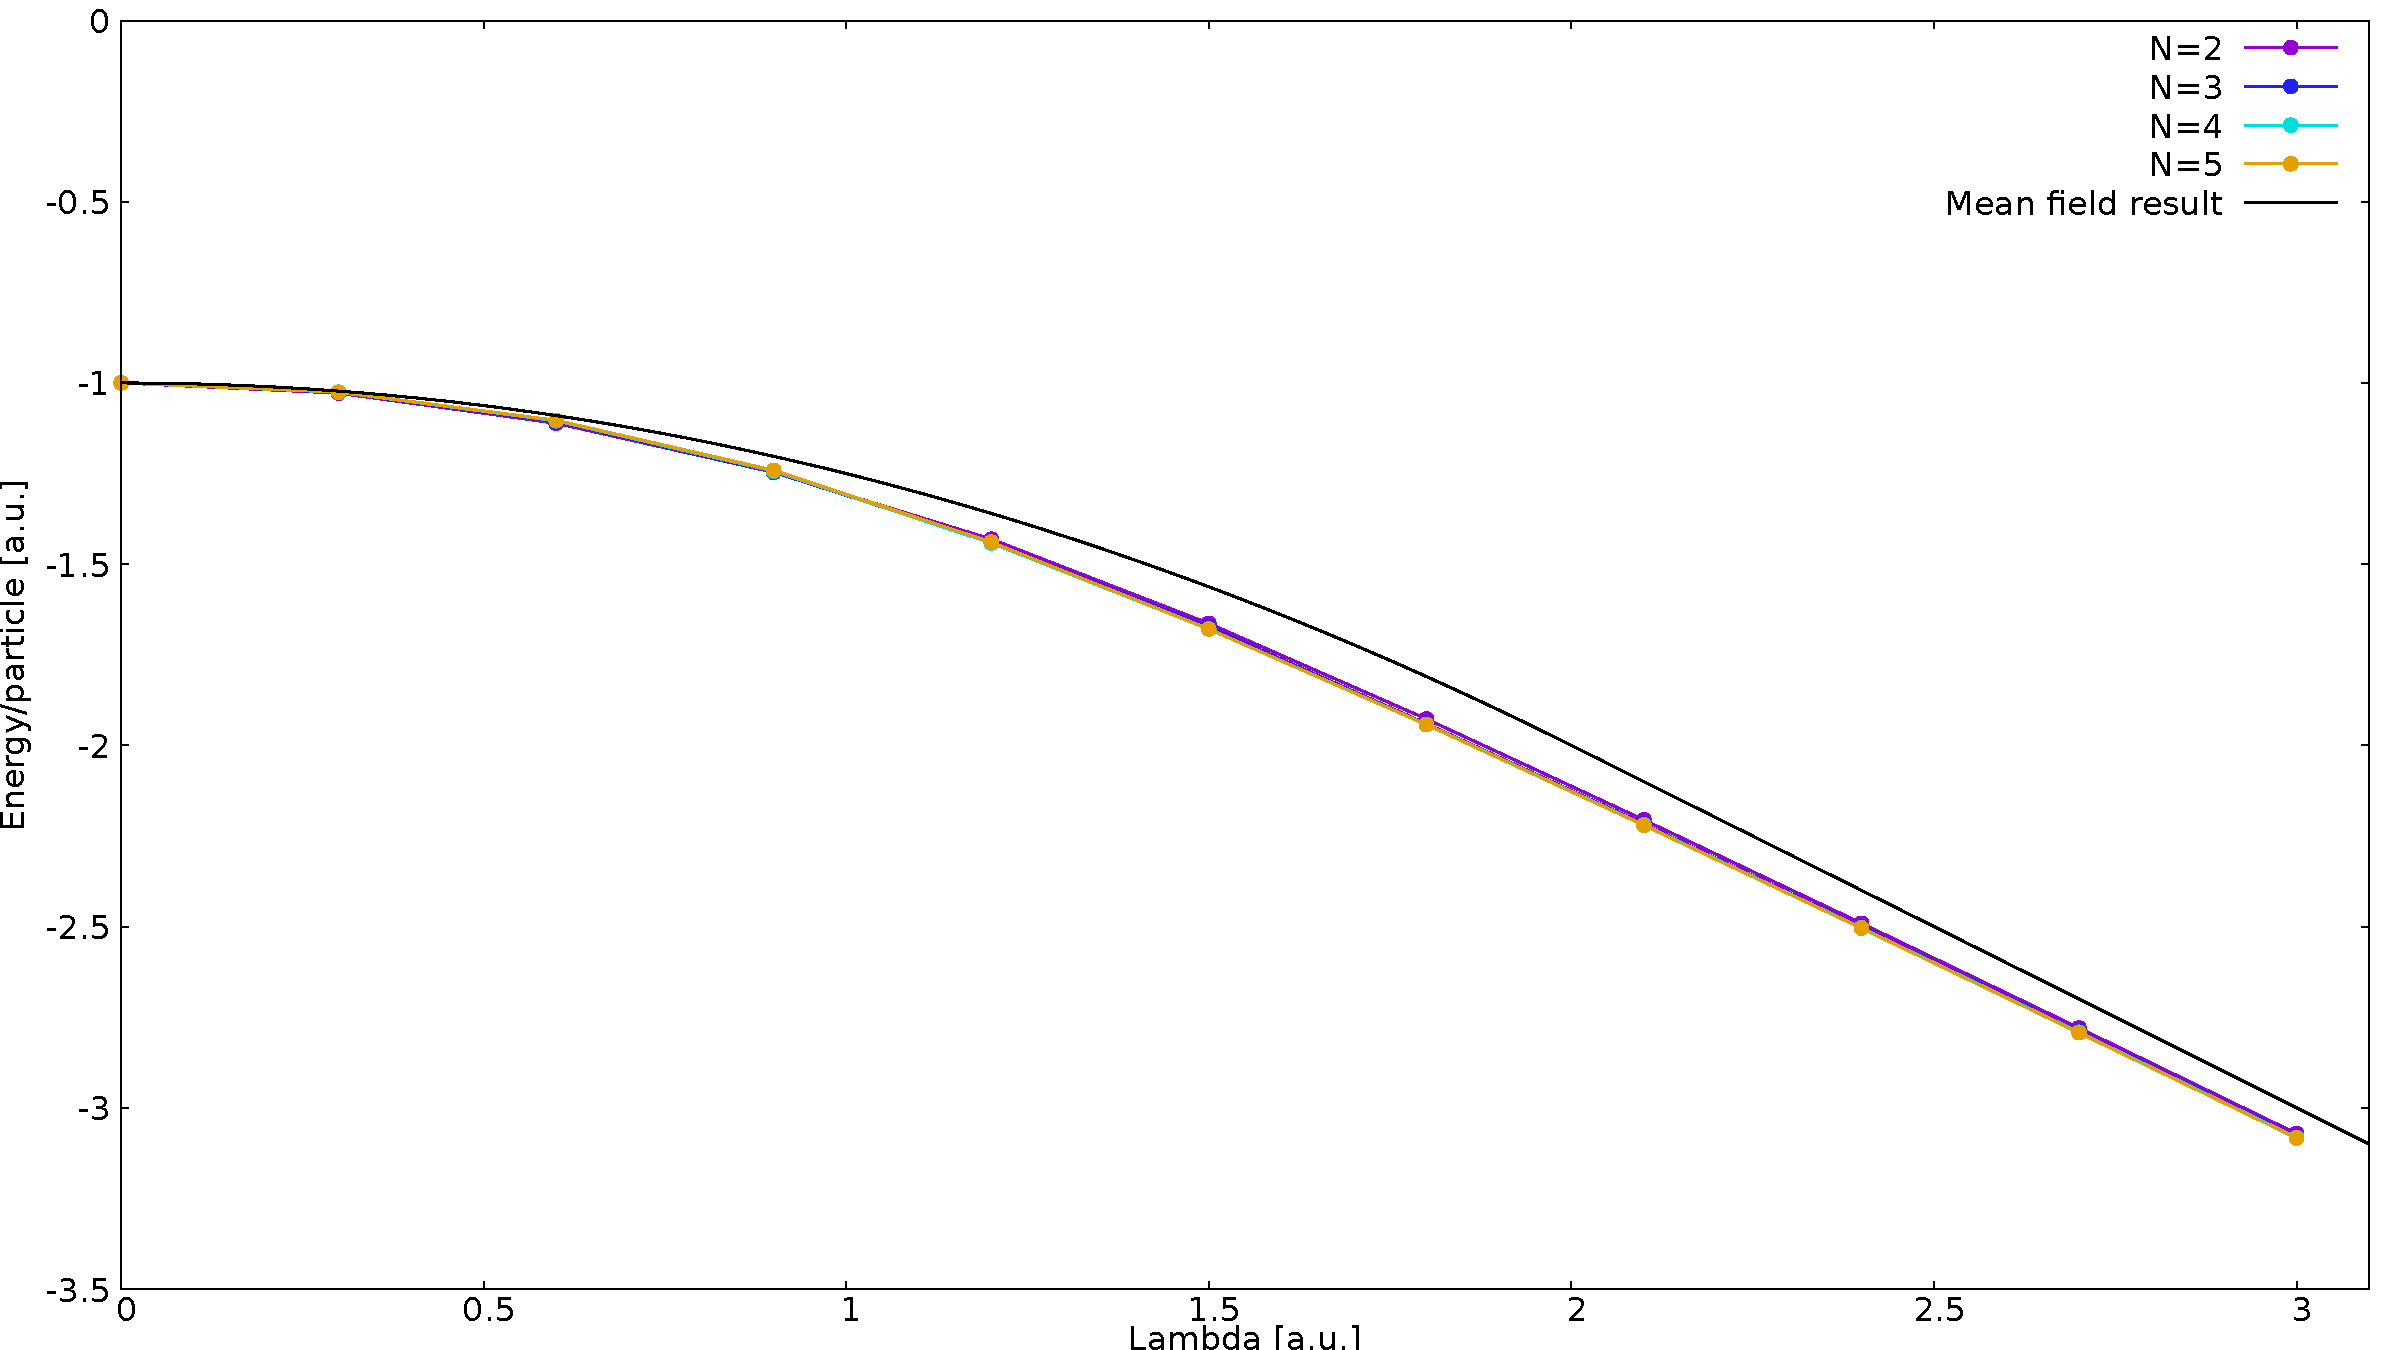
\includegraphics[scale=0.3]{eigval_vs_lambda.pdf}
	\caption{Hamiltonian ground states for different values of (starting) $N$ vs $\lambda$.}
	\label{figure_lambdas}
\end{figure}


The $H_N$ hamiltonian is composed by two parts: the first one represents the z-component spin interactions with an external magnetic field $\lambda$ (more precisely, the interaction with the z-component of such a field) while the second part is that of an antiferromagnetic system.

Before going further, let us adopt a change of notation: "$\pm$1/2" spins will be denoted using "$\pm$1".

The ground state of the first part alone is a state in which all the z-components of the spins are directed as the external field but have opposite orientation. The ground state of the second system (in absence of an external field) is that where all the spins alternate their x-components, thus reaching a minimum of the energy. This state is degenerated since there are two configurations that make it possible: one where the "first" spin has x-component equal to +1 (and all the others have their x-components alternated: so $\sigma_x^{i=2} = -1, \sigma_x^{i=3} = +1$ and so on), the other having the first x spin component set to +1.

The second energy state for the first system is that when one single spin is oriented in the same way as the external field: this state has degeneration equal to the number of particles $N$ since it can be achieved in turning one single particle having N different particles to handle. The second energy state of the second subsystem is reached when one single interaction "breaks the alternance chain", for example in the chain $\sigma_x^{i=1} = -1, \sigma_x^{i=2} = +1, \sigma_x^{i=3} = -1, ... , \sigma_x^{i=2k-1} = -1, \sigma_x^{i=2k} = -1, \sigma_x^{i=2k+1} = +1, ...$ the $\sigma_x^{i=2k} = -1$ is the opposite of that expected, and after it all the others are reversed (so that one single interaction term is reversed). Straightforward, the degeneration of this state is $N-1$ since there can be $N-1$ different interactions that can be changed to pass from the ground state to the second one.

%The spectrum of the system represent the energy levels accessible by the system itself. When the $\lambda$ parameter is equal to 0 the system is described only by the second part of the hamiltonian thus showing the behaviour aforementioned with the first two eigenvalues being degenerated. With increasing $\lambda$ the system is described more likely by the first part of the hamiltonian, thus the first eigenvalue tends not to be degenerated. While passing from one to another a phase trainsition occurs. Specifically, it is a quantum phase trainsition because the system has a quantum nature.

In the figure, the ground state for each system can be seen. One can use these estimations (assuming they represent the "truth") to verify how good the mean field approximation is. It seems that for $\lambda \simeq 0$ the MF function for the \textit{energy per particle} in the ground state is near the values of \textit{real-space RG}, then for $\lambda \simeq 1$ the functions start to be different; anyway, the trend of them seems to make them nearer when further increasing $\lambda$: this fact can make us think that the MF approximation is good for small and large values of $\lambda$, while for "critical values" of it (where we expect there is a phase transition) the MF approximation is not good.

\section*{Self-evaluation}
In this task I learned how to implement a \textit{real-space RG} procedure for a system made of $N$ 1/2-spin particles system.

\subsection*{Correctness}

My program does what is expected to do, but as aforementioned, it works reasonably fast only for $N \leq 5$; for larger values, it takes more than four hours to run.

There are no compilation problems.

Pre- and post-conditions and checkpoints are not used so much due to the large amount of time they require to be implemented (compared to the time we have to do the task).

\subsection*{Stability}

There are loops made on non integers variables, but there is no specific check that can lead to "weird errors".

Maybe some memory error can arise if the space dimension $d$ or the number of particles $N$ (or even both parameters) become too large due to the fact that the matrix dimension goes as $d^{2N}$.

\subsection*{Accurate discretization}

There is no particular discretization issues.

\subsection*{Flexibility}

I tried to comment as much as possible the code so to have a clear and understandable code.

\subsection*{Efficiency}

Diagonalization routine is not implemented by hand. For what concerns memory and time usage, they depend on the parameters passed.

\end{document}